%%%%%%%%%%%%%%%%%%%%%%%%%%%%%%%%%%%%%%%%%%%%%%%%%%%%%%%%%%%%%%%%%%%%%%%%%%%%%%%%%%%%%%%%%%%%%%%%%%%%%%%%%%%%%%%%%%%%%%%%%%%%%%%%%%%%%%%%%%%%%%%%%%%%%%%%%%%
% This is just an example/guide for you to refer to when submitting manuscripts to Frontiers, it is not mandatory to use frontiers.cls nor frontiers.tex  %
% This will only generate the Manuscript, the final article will be typeset by Frontier after acceptance.                                                 %
%                                                                                                                                                         %
% When submitting your files, remember to upload this *tex file, the pdf generated with it, and all the figures.
%%%%%%%%%%%%%%%%%%%%%%%%%%%%%%%%%%%%%%%%%%%%%%%%%%%%%%%%%%%%%%%%%%%%%%%%%%%%%%%%%%%%%%%%%%%%%%%%%%%%%%%%%%%%%%%%%%%%%%%%%%%%%%%%%%%%%%%%%%%%%%%%%%%%%%%%%%%

%%% Version 2.4 Generated 2014/03/12 %%%
%%% You will need to have the following packages installed: datetime, fmtcount, etoolbox, fcprefix, which are normally inlcuded in WinEdt. %%%
%%% In http://www.ctan.org/ you can find the packages and how to install them, if necessary. %%%

\documentclass{frontiersENG} % for Engineering articles
%\documentclass{frontiersSCNS} % for Science articles
%\documentclass{frontiersHLTH} % for Health articles
%\documentclass{frontiersFPHY} % for Physics articles

%\setcitestyle{square}
\usepackage{url,lineno}
\usepackage{tcolorbox}

\linenumbers


% Leave a blank line between paragraphs in stead of using \\

\copyrightyear{}
\pubyear{}

\def\journal{Genetics}%%% write here for which journal %%%
\def\DOI{}
\def\articleType{Review Article}
\def\keyFont{\fontsize{8}{11}\helveticabold }
\def\firstAuthorLast{Thompson {et~al.}} %use et al only if is more than 1 author
\def\Authors{Jeffrey A. Thompson\,$^{1}$, Clare Bates Congdon\,$^{1,*}$}
% Affiliations should be keyed to the author's name with superscript numbers and be listed as follows: Laboratory, Institute, Department, Organization, City, State abbreviation (USA, Canada, Australia), and Country (without detailed address information such as city zip codes or street names).
% If one of the authors has a change of address, list the new address below the correspondence details using a superscript symbol and use the same symbol to indicate the author in the author list.
\def\Address{$^{1}$Department of Computer Science, University of Southern Maine, Portland, ME, USA}
% The Corresponding Author should be marked with an asterisk
% Provide the exact contact address (this time including street name and city zip code) and email of the corresponding author
\def\corrAuthor{Clare Bates Congdon}
\def\corrAddress{Department of Computer Science, University of Southern Maine, 96 Falmouth Street, Portland, ME, 04104-9300, USA}
\def\corrEmail{congdon@usm.maine.edu}

% \color{FrontiersColor} Is the color used in the Journal name, in the title, and the names of the sections.


\begin{document}
\onecolumn
\firstpage{1}

\title[Developments in comptutational CRM prediction]{Developments in computational cis-regulatory module prediction}
\author[\firstAuthorLast ]{\Authors}
\address{}
\correspondance{}
\extraAuth{}% If there are more than 1 corresponding author, comment this line and uncomment the next one.
%\extraAuth{corresponding Author2 \\ Laboratory X2, Institute X2, Department X2, Organization X2, Street X2, City X2 , State XX2 (only USA, Canada and Australia), Zip Code2, X2 Country X2, email2@uni2.edu}
\topic{}% If your article is part of a Research Topic, please indicate here which.

\maketitle

%%%%%%%%%%%%%%%%%%%%%%%%%%%%%%%%%%%%%%%%%%%%%%%%%%%%%%%%%%%%%%%%%%%%%%%%%%%%%%%%%%%%%%%%%%%%%%%%%%%%%%%%%%%%%%%%%%%%%%%%%%%%%%%%%%%%%%%%%%%%%%%%%%%%%%%%%%%%%%%%%%%%%%%%%%%%%%%%%%%%%%%%%%%%%%%%%%%%%%%%%%%%%%%%%%%%%%%%%%%%%%%%%%%%%%%
%%% The sections below are for reference only.
%%%
%%% For Original Research Articles, Clinical Trial Articles, and Technology Reports the section headings should be those appropriate for your field and the research itself. It is recommended to organize your manuscript in the
%%% following sections or their equivalents for your field:
%%% Abstract, Introduction, Material and Methods, Results, and Discussion.
%%% Please note that the Material and Methods section can be placed in any of the following ways: before Results, before Discussion or after Discussion.
%%%
%%%For information about Clinical Trial Registration, please go to http://www.frontiersin.org/about/AuthorGuidelines#ClinicalTrialRegistration
%%%
%%% For Clinical Case Studies the following sections are mandatory: Abstract, Introduction, Background, Discussion, and Concluding Remarks.
%%%
%%% For all other article types there are no mandatory sections.
%%%%%%%%%%%%%%%%%%%%%%%%%%%%%%%%%%%%%%%%%%%%%%%%%%%%%%%%%%%%%%%%%%%%%%%%%%%%%%%%%%%%%%%%%%%%%%%%%%%%%%%%%%%%%%%%%%%%%%%%%%%%%%%%%%%%%%%%%%%%%%%%%%%%%%%%%%%%%%%%%%%%%%%%%%%%%%%%%%%%%%%%%%%%%%%%%%%%%%%%%%%%%%%%%%%%%%%%%%%%%%%%%%%%%%%

\begin{abstract}
Dozens of approaches have been created to predict cis-regulatory
modules (CRMs). Two separate reviews, in 2009 and 2010 compared many
of these tools and identified the most promising approaches, as well
as the need for improvement. Since those reviews were published, a
number of new methods have been developed that offer significant
advantages over what came before. Additionally, breakthroughs in high
throughput biological experimental techniques have occurred that may
mitigate or complement the need for computational prediction. In this
work we examine the developments in CRM prediction since that time and
look at the capabilities of the latest generation of tools and
techniques.

%As a primary goal, the abstract should render the general significance and conceptual advance of the work clearly accessible to a broad readership. References should not be cited in the abstract.

\tiny
 \keyFont{ \section{Keywords:} cis-regulatory module, CRM, gene regulation, epigenetic, motif, computational prediction, gene regulatory network, GRN} %All article types: you may provide up to 8 keywords; at least 5 are mandatory.
\end{abstract}

\section{Introduction}
\label{section:intro}
Multicellular organisms exhibit complex patterns of differential gene
expression to enable the varied roles of their various tissues and
organs. Still other patterns of expression are critical to the initial
development of the organism and the organization of its body
plan. Disruption of these patterns can occur through mutation and
exposure to toxins, leading to cancer and other diseases. Therefore,
much research has been devoted to understanding how these key
differential expression patterns are maintained.

A cell has many opportunities to regulate a gene, but a key element is
the set of cis-regulatory modules (CRMs) that control the gene's
transcription. A cis-regulatory module (CRM) is a region of noncoding
DNA that groups together specific transcription factor binding sites
(TFBSs) that together affect gene expression (see Box
\ref{box:regpathways}). This combinatory organization allows a
relatively small number of transcription factors to participate in the
complex differential expression patterns of a larger number of
genes. Genes may be regulated by multiple CRMs that control their
expression in various contexts, making knowledge of CRMs an important
part of understanding gene regulatory networks and disease.

In the past, biological elucidation of regulatory function was a slow
and arduous process. Because of this, computational tools were
developed to focus biological experiments on high confidence areas for
investigation. Recent developments in high-throughput techniques have
made volumes of experimental data available, such as DNase-Seq,
FAIRE-Seq, and ChIP-Seq, indicating various regulatory pathways, such
as chromatin accessibility, histone modification, and transcription
factor binding (see Box \ref{box:regpathways}). Some have suggested
that such data may supplant the need for computational inference
\cite{Hardison2012}. Nevertheless, these experimental data cannot yet
tell the whole story. They are limited to a particular cell type, at a
particular time, under particular conditions. Publically available
data have been generated for a limited number of genomes and cell
types and are not yet available for most regulatory proteins, while
the cost of generating such comprehensive epigenetic data will likely
remain out of reach for many labs for some time to come. Additionally,
these high-throughput assays are not capable of conclusively
establishing regulatory function. Therefore, computational tools
remain an important part of learning about CRMs, perhaps in
conjunction with this new high-throughput data.

In this review we will briefly discuss the development of the
computational prediction of CRMs, as well as biological methods. The
most recent review of CRM prediction techniques was in 2012
\cite{Hardison2012}. However, the focus of that review was on
biological methods of predicting regulatory regions and its discussion
of computational methods was focused primarily of general differences
between approaches, rather than specific tools that are publically
available to researchers. Furthermore, there have been a number of
important developments in prediction methods that were either
published after that review, or were not covered in it. The emphasis
of this review will be on developments in CRM prediction that are
available to the public. Earlier reviews provide a comprehensive look
at older methods \cite{Elnitski2006}, \cite{Loo2009},
\cite{Su2010}. Although useful, one issue often overlooked in earlier
reviews is that the various methods are often designed with a
particular use in mind, but the experimental design used to compare
methods tends to favor those that solve just one aspect of the
problem. Our focus will be to provide information on the problems
particular methods were designed to solve to better enable researchers
to pick the tool appropriate for the work in hand.

\begin{tcolorbox}[title=Box 1 | Pathways of Pre-Transcriptional Regulation]
  \setlength{\parskip}{.5em}
  \label{box:regpathways}

  What follows is a description of some of the major pathways of
  pre-transcriptional regulation. Transcription is regulated in many
  ways, and this list cannot be considered comprehensive.

  \textit{Transcription factor binding:} transcription factors are
  proteins that bind to DNA and regulate the transcription of a
  gene. The regulation can happen through a variety of means, such as
  recruiting poylmerase II, signaling that transcription should begin,
  or interfering in some way with other transcription factors. \par

  \textit{Histone modification:} DNA is organized into nucleosomes,
  which consist of DNA wrapped around histone protein complexes. Tails
  of the histone proteins extend from the nucleosome and these tails
  can be modified by the addition of members of acetyl or methyl
  chemical groups (see Fig. \ref{fig:epigenetic}). These modifications
  are still under investigation but have been observed to play a role
  in gene regulation. \par

  \textit{Chromatin accessibility:} Chromatin is the DNA in
  combination with the proteins it is bound to. It has a highly
  organized state in order control the vast length of DNA managed in
  the small nucleus of the cell. Active regions of chromatin often
  need to be less compact then inactive regions, in order to be more
  accessible to ligands (such as transcription factors). Therefore,
  chromatin accessibility can indicate regions more likely to
  function in gene regulation. \par

  \textit{DNA Methylation:} DNA methylation involves the attchment of
  molecules from the methyl functional group to DNA nucleotides. This
  leads to the compaction of the genome at methylated regions and the
  repression of gene transcription. Methylation also plays other
  regulatory roles in the genome, such as the repression of
  transposons \cite{Espada2010}, \cite{Robertson2000}.\par
\end{tcolorbox}
% This box needs some work, but I think I want something like this in here.

\section{Cis-Regulatory Modules}
\label{section:crms}
A CRM is a region of DNA that can be bound by a limited set of
transcription factors under specific conditions to regulate the
expression of a gene. The concept of CRMs is important, in part
because transcription factor binding sites are short (approximately
6--20bp) and degenerate (a transcription factor can bind to a variety
of sites). Because of this, a transcription factor could theoretically
bind in many locations across the genome. It is in combination with
other factors and under the correct condition that transcription
factors bind to CRMs and affect gene expression. By identifying CRMs,
the specificity of predicted transcription factor binding sites can be
increased and the combinatorial control of a gene better
understood. Therefore, identification of CRMs is critical to revealing
the regulatory network that determines when a gene is active.

\subsection{Types of CRMs}
\label{section:crmtypes}
There are a number of different types of CRMs, which are classified by
their regulatory effect:
\begin{itemize}
\item{\textit{Promoters}. Eukaryotic protein-coding gene promoters are
  a region of noncoding DNA that enables RNA polymerase II to initiate
  transcription of the gene. The region is usually located close to
  the transcription start site (TSS) \cite{Taher2013}. The promoter is
  sometimes divided into two areas: the core promoter and the proximal
  promoter \cite{Taher2013}, \cite{Butler2002}. Both are bound by
  transcription factors, but the core promoter is the minimal region
  required for transcription. Core promoter studies have shown that
  most genes have multiple promoters driving alternative transcription
  \cite{Sandelin2007}. }

\item{\textit{Enhancers}. Enhancers are regions of noncoding DNA that
  control the conditions under which a gene is transcribed. They
  target a promoter and increase the probability of transcription
  \cite{Walters1995}. They can be located distally from the gene and
  some function regardless of orientation \cite{Blackwood1998},
  \cite{Laimins1984}. However, in other cases orientation matters
  \cite{Hozumi2013}. Enhancers are structurally similar to proximal
  promoters \cite{Maston2006}.}

\item{\textit{Silencers}. Silencers also control the conditions under
  which a gene is transcribed but, contrary to enhancers, they act to
  repress the transcription of a gene \cite{Ogbourne1998}. Many
  silencers are similar to enhancers in their relative independence of
  location and orientation, but others are not. There are a number of
  different types of silencers \cite{Ogbourne1998}, some of which
  interfere with transcription factors, the chromatin structure, or
  the formation of the transcription initiation complex with
  polymerase II. Also, there is evidence that an enhancer may switch
  to a silencing function \cite{Jing2008}.}

\item{\textit{Insulators}. Insulators act to stop regulatory effects
  from one region affecting another region. This might involve
  blocking an enhancer, so that it does not affect a particular
  promoter, or blocking the spread of heterochromatin (compact,
  silenced chromatin) \cite{Ghirlando2012}.}
\end{itemize}

\subsection{Characteristics of CRMs}
\label{section:crmcharacteristics}
Numerous studies have revealed properties of CRMs that differentiate
them from surrounding sequence. These characteristics are exploited by
CRM prediction methods to identify regions of DNA sequence associated
with regulatory function.
\begin{itemize}

\item{\textit{Clustering}. CRMs are composed of clusters of
  transcription factor binding sites. Although individual sites can
  occur at random, this is significantly less likely to happen for
  clusters of binding sites \cite{Wagner1999}. Therefore, clusters of
  transcription factor binding sites may indicate a CRM. Clustering
  can be divided into two basic types:
  \begin{itemize}
    \item{\textit{Homotypical clusters}. The clusters are composed of
      a number of repeats of the same basic binding site. For a while
      this was thought to possibly be a general CRM feature, but it
      turns out to be true of only a subtype of CRMs \cite{Li2007}.}
    \item{\textit{Heterotypical clusters}. The clusters contain a
      binding sites for a number of different transcription
      factors \cite{Roth2007}.}
  \end{itemize}
}

\item{\textit{Conservation}. CRMs have been shown to be more highly
  conserved than flanking regions \cite{Kwon2011},
  \cite{Li2007}. Additionally, TFBSs within CRMs can exhibit an even
  higher level of constraint \cite{Kwon2011}. Because these regions
  are functionally important, purifying selection has the effect of
  conserving them. This is not to say that all CRMs will be conserved
  across diverse species. It is likely that many lineage specific CRMs
  exist, possibly contributing to species diversity. The frequency of
  lineage specific CRMs is not known.}

\item{\textit{GC-content}. Some CRMs have been shown to have elevated
  GC-content compared to other noncoding sequence \cite{Li2007},
  \cite{Saxonov2006}.}

\item{\textit{Motif Synergy}. CRMs are composed of specific groups of
  transcription factor binding sites. Transcription factors bound to
  these sites exhibit synergistic effects (the degree of regulation is
  greater than the contribution of a particular factor). These
  transcription factors may need to be certain distances from or
  orientations to each other. Therefore, the relationship of specific
  binding sites can be used in recognizing CRMs.}

\item{\textit{Size}. The largest database of biologically validated
  CRMs is RedFly \cite{Gallo2011}, which contains hundreds of
  validated functional CRMs in \textit{Drosophila}, which have been
  reduced to minimal size required to regulate the gene. An
  examination of these CRMs showed the length of CRMs to be variable
  (most were between 100 and 2100 bp in length with an average of
  760bp) \cite{Li2007}. The size characteristics of CRMs in other
  genomes may be different.}

\item{\textit{Epigenetic Properties}. A number of biochemical marks
  are associated with active CRMs. These include chromatin
  accessibility, certain histone modifications, and methylation
  patterns \cite{Calo2013}, \cite{Bannister2011}, \cite{Encode2011},
  \cite{Cheng2011}. Of course, these markers of CRMs are not at the
  sequence level, where most past research has been focused. There
  have recently been concerted efforts to map all known epigenetic
  marks to a few genomes.}

\end{itemize}

\begin{figure}[ht!]
\centering
  \vspace{-10pt}
  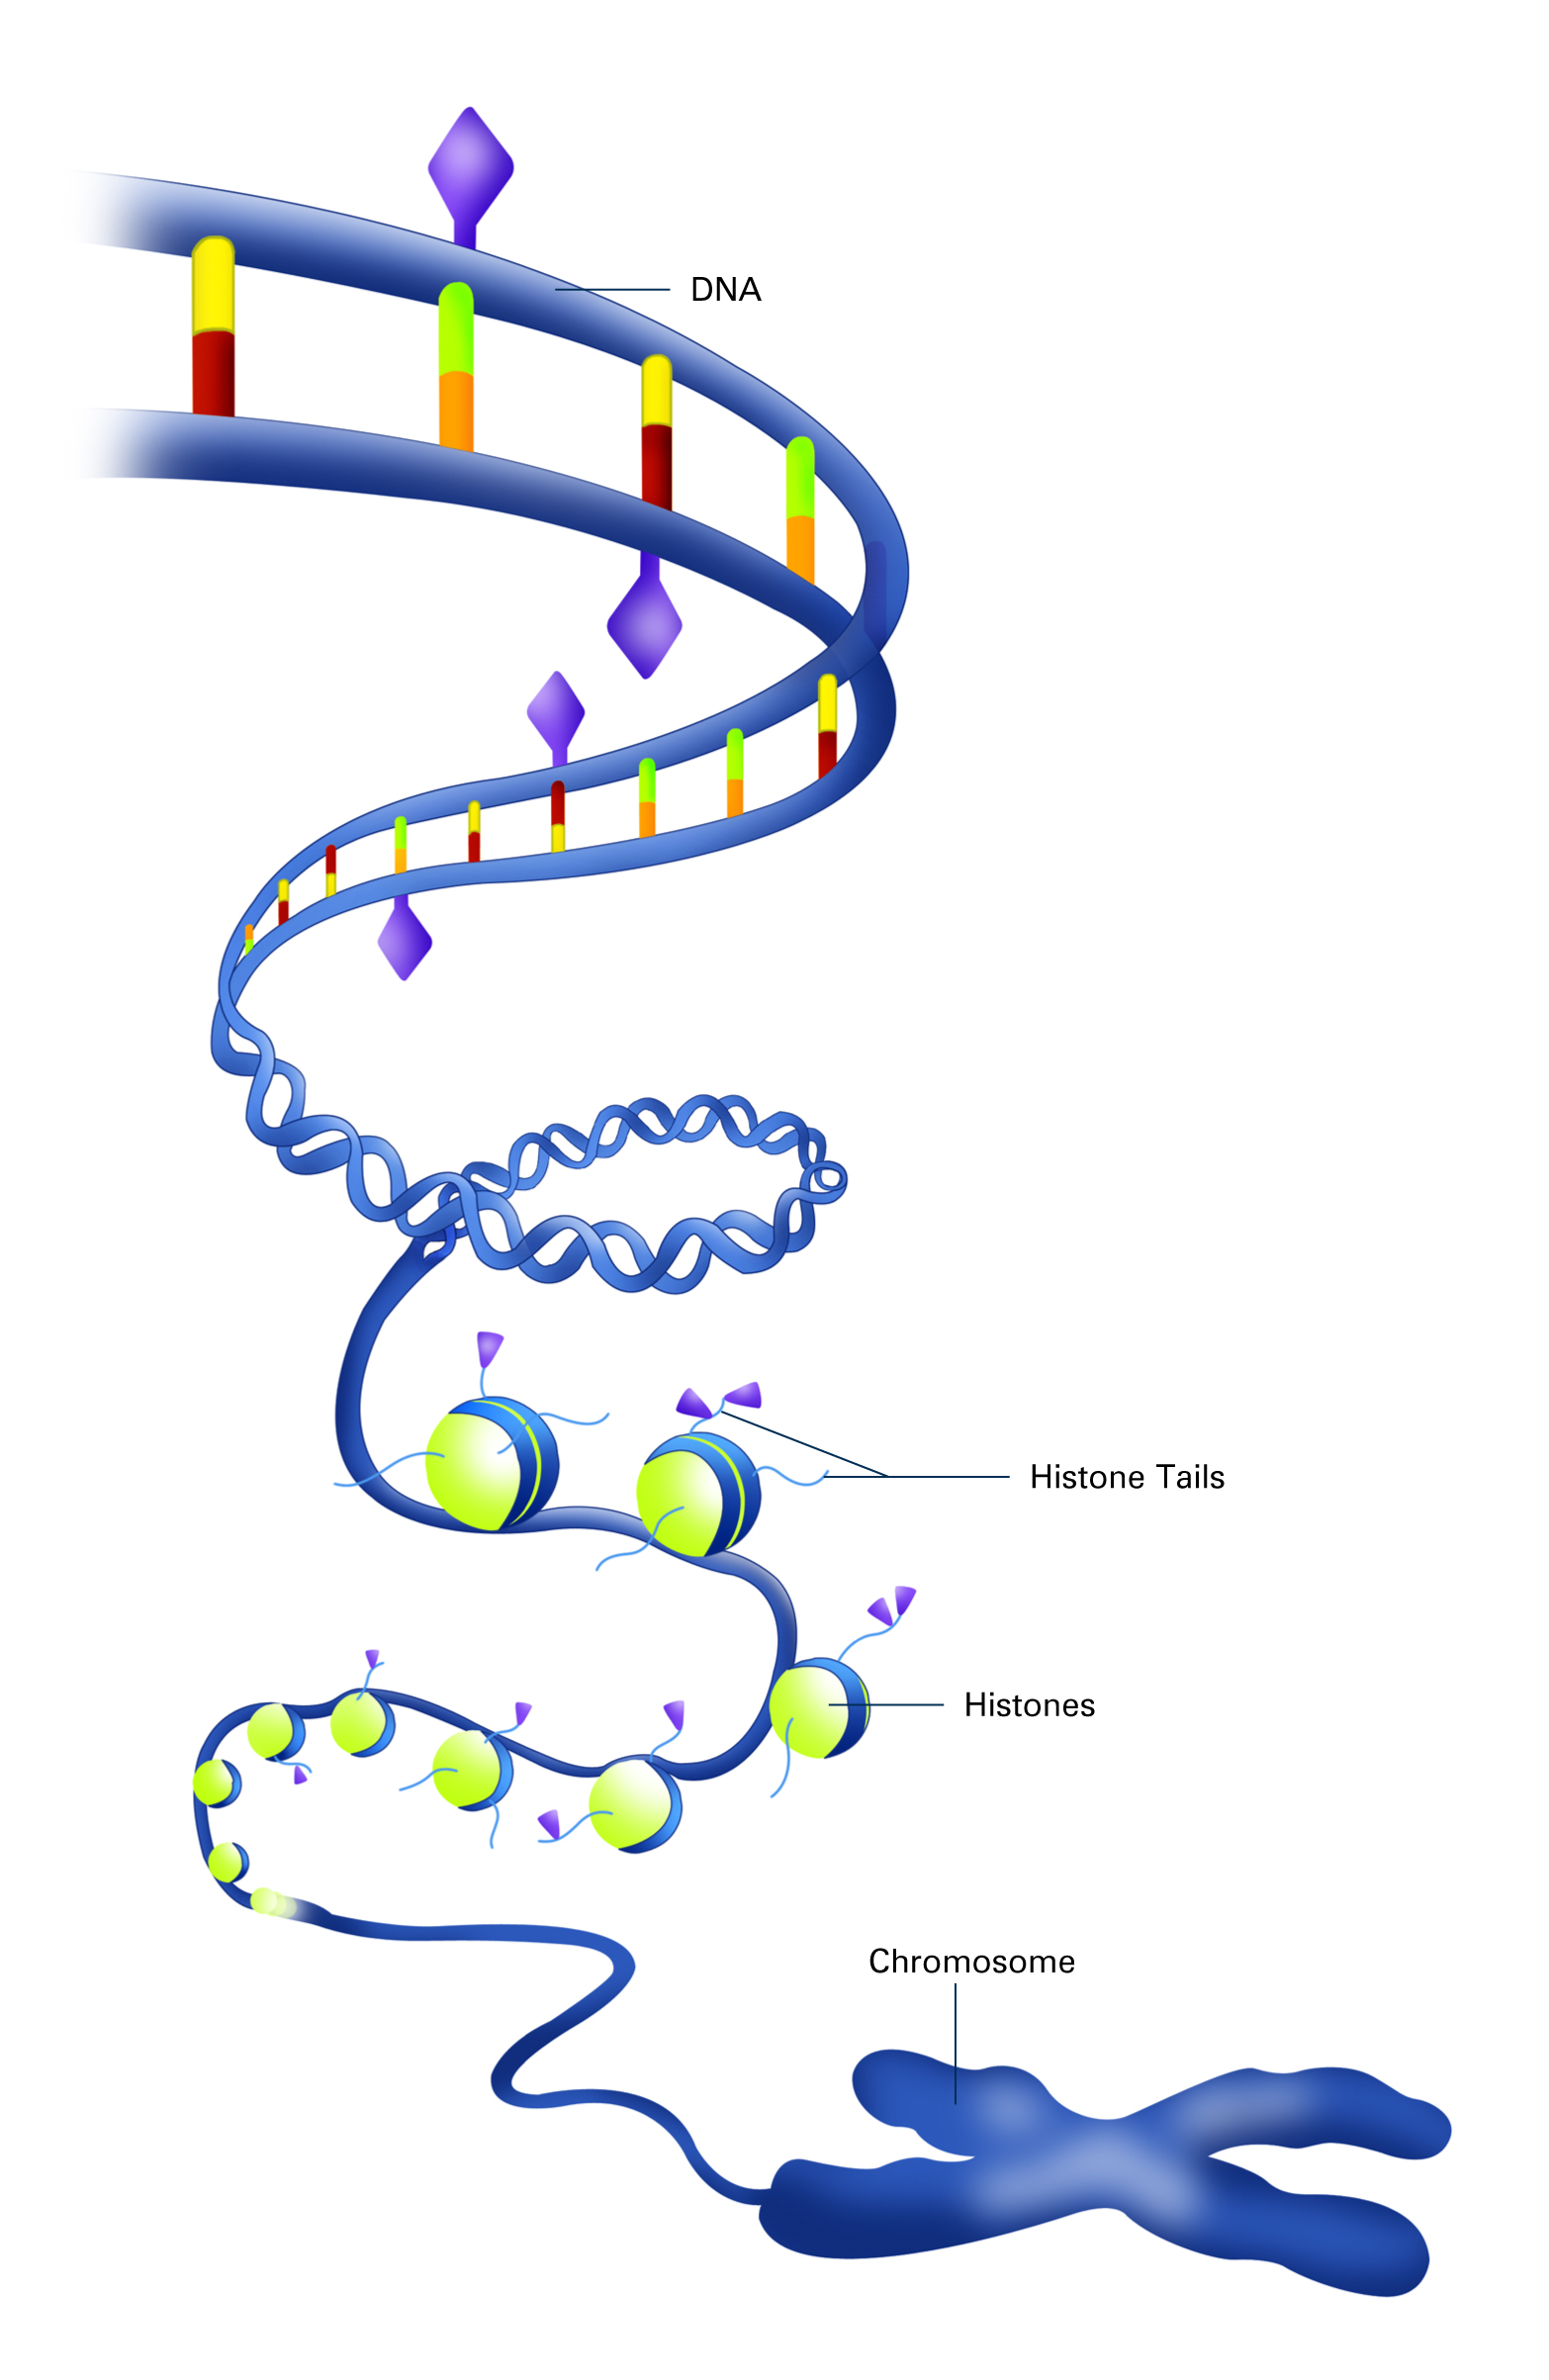
\includegraphics[width=3.5in]{epigenetic.jpg}
  \caption{DNA is organized into nucleosomes (regions of DNA wrapped
    around histone proteins). Modifications to the tails of these
    histones, such as the addition of members of the methyl or acetyl
    groups, can affect the regulation of genes (shown as
    triangles). Certain marks are known to be associated with
    cis-regulatory modules. Methyl groups might also be attached
    directly to the DNA, repressing transcription of a gene (shown as
    diamonds). Image courtesy of NIGMS, provided by Crabtree \&
    Company.}
  \label{fig:epigenetic}
\end{figure}

The characteristics of CRMs listed above are those that have generally
been found to be useful in in distinguishing CRMs from background
sequences. There may be others. 

\section{Computational Prediction of CRMs}
\label{section:compprediction}
As early as 1985, a computational tool had been written to detect
eukaryotic gene promoters \cite{Claverie1985}. This early tool
searched for manually defined patterns of sequences thought specific
to heatshock and glucocorticoid regulated promoters. Development of
additional techniques for promoter identification followed, such as
one that analyzed the density of known transcription factor binding
patterns in promoters vs. non-promoters and built a promoter
recognition profile \cite{Prestridge1995} that could be used to
recognize similar promoters and another \cite{Chen1997}, which
analyzed the density of 5-10bp strings in known promoters in order to
build a profile.

Following those tools, a number of approaches were developed to
identify clusters of position weight matrices (PWMs). PWMs capture the
information from multiple binding sites for a transcription factor in
an attempt to describe the variety of sites a transcription factor
might bind to (see Table \ref{table:arntPWM}). A PWM shows how often a
given base was seen at a particular position in the binding
sites for a transcription factor. PWMs were first used to search for
transcription factor binding sites in 1996
\cite{Fickett1996}. However, they were soon used to search for CRMs
\cite{Wasserman1998}, often by searching for clusters of particular
PWMs that might regulate under a specific context. Since that time,
various methods of searching for clusters of PWMs has been the
predominant method of predicting CRMs computationally \cite{Elnitski2006},
\cite{Loo2009}, \cite{Su2010}.

\begin{table}[!t]
\textbf{\refstepcounter{table}\label{table:arntPWM} Table \arabic{table}.}{ Position Weight Matrix for Arnt (Aryl hydrocarbon receptor nuclear translocator): The log-likelihood of the occurence of each base at each position in the binding site is shown. }

\processtable{ }
{\begin{tabular}{ccccccc}\toprule
 & \textbf{1} & \textbf{2} & \textbf{3} & \textbf{4}  & \textbf{5} & \textbf{6}\\
\midrule
A & -0.31 & 1.88 & -4.70 & -4.70 & -4.70 & -4.70 \\
C & 1.64 & -4.70 & 1.96 & -4.70 & -4.70 & -4.70 \\
G & -4.70 & -2.12 & -4.70 & 1.96 & -4.70 & 1.96 \\
T & -4.70 & -4.70 & -4.70 & -4.70 & 1.96 & -4.70 \\
\botrule

\end{tabular}}{}
\end{table}

Even the first method to use PWMs anticipated the need for more
information and recommended using conservation analysis when the data
were available \cite{Wasserman1998}. As noted in Section
\ref{section:crms}, many CRMs are conserved by purifying
selection. Therefore, it is possible to use conservation to help
identify such CRMs. For a while, it was difficult to find sufficient
orthologous data to use, and most of the early tools did not use
conservation (e.g. \cite{Sinha2003}, \cite{Frith2003}). Nevertheless,
it was soon incorporated as a filter in a number of tools
(e.g. \cite{Sinha2004}, \cite{Sinha2007}).

Conservation can also be used as the main feature in CRM detection
(rather than as an additional filter). Methods of this sort were also
developed around the same time \cite{Kolbe2004}. Neither clustering
nor conservation can provide information about the context of when and
where the gene a CRM regulates is active, unless the binding sites
predicted are for transcription factors known to be active in a
particular context. They simply identify regions that are more likely
to regulate the gene and possibly suggest the other genes involved in
that regulation.

By 2010, several dozen different methods had been developed for CRM
prediction. One independent assessment using benchmark data
\cite{Su2010} found that the Regulatory Potential method
\cite{Kolbe2004} performed the best on the human genome, although this
method does not identify binding sites within the CRM. The method
compares two-way alignments of human and mouse DNA and classifies
alignments based on whether or not short fixed sequences in the
alignments are more typical of regulatory or neutral regions based on
statistical models. For \textit{Drosophila}, the most successful
method was MorphMS \cite{Sinha2007}, which combines clustering of PWMs
and conservation to make predictions, with the conservation measured
as conserved binding sites, rather than the more typical
alignments. Despite the application of increasingly sophisticated
techniques, no one method had emerged that could reliably predict
functional CRMs from DNA sequence data alone \cite{Su2010}. Most
methods that depend primarily on detecting clusters of binding sites
using PWMs rely on prior knowledge of processes that the CRMs being
searched for might be involved in so that suitable PWMs can be
selected. This limits them to detecting CRMs controlling the gene's
known pathways. Furthermore, CRMs do not always exhibit tight
clustering of binding sites. Methods that are capable of selecting the
PWMs that might regulate a gene from a larger library had not yet seen
much success \cite{Loo2009}. Neither had \textit{de novo} approaches
that did not rely on PWMs \cite{Su2010}.

\section{High-Throughput Biological Screening}
\label{section:hts}

Most of the approaches developed prior to 2010 made CRM predictions
based on the DNA sequence. However, there are numerous epigenetic
markers associated with gene regulation \cite{Bernstein2007}, which
can be tested with an array of high-throughput techniques. Until
relatively recently, the time and expense associated with assays for
these marks limited their use. However, breakthroughs in
high-throughput techniques have made large amounts of epigenetic data
available. Therefore, interest has grown in using these marks to
indicate regulatory regions biologically. A few large efforts have
started to map regulatory markers genome-wide. The ENCODE consortium
has used many of these assays across the human genome
\cite{Dunham2012} and these data are publically available through the
UCSC Genome Browser \cite{Rosenbloom2013}, \cite{Kent2002}. Similar
projects exist for \textit{Drosophila melanogaster} and
\textit{Caenorhabditis elegans} \cite{Celniker2009}, and for
\textit{Mus musculus} \cite{Stamatoyannopoulos2012}.

Here, we will briefly describe some of the major assays used for
high-throughput analysis of epigenetic data. Although there are other
methods available, these will serve to illustrate the types of data
that are available.

\subsection{ChIP-seq}
Chromatin immunoprecipitation followed by sequencing (ChIP-seq)
identifies proteins bound to DNA \cite{Kim2007}, \cite{Barski2007},
\cite{Ren2000}. This can be directed at identifying transcription
factors bound to chromatin, histone modifications (that mark
regulatory regions), RNA polymerase II binding, and more. One
limitation of this technique is its requirement for an antibody that
binds to the protein targeted by the assay. Antibodies are not
available for all regulatory proteins.

\subsection{DNase-seq}
DNase hypersensitive site sequencing (DNase-seq) identifies regions
where the DNase I enzyme digests chromatin more readily
\cite{Crawford2006} (which are then sequenced with high-throughput
techniques). These regions of open chromatin more accessible to
regulatory proteins. Active regulatory regions, bound by transcription
factors, form DHSs \cite{Cockerill2011}, making them a useful tool in
identifying candidate regulatory regions.

\subsection{FAIRE-seq}
Formaldehyde assisted isolation of regulatory elements followed by
sequencing (FAIRE-seq) \cite{Giresi2009}, \cite{Giresi2007} is another
technique for indetifying regions of accessible
chromatin. Formaldehyde cross-links more efficiently to nucleosomes,
allowing nucleosome-free DNA to be identified. These regions are
associated with regulatory activity.

\subsection{RRBS}
Reduced representation bisulfite sequecing (RRBS), is a method that
can be used to identify methylated cytosine. Methylated DNA is often
repressed, reducing transcription. The chromatin is treated with
sodium bisulfite, converting unmethylated cytosine to uracil
\cite{Frommer1992}. The remaining cytosines are methylated. The
reduced representation refers to the fact that the genome is
fragmented and selected for regions with high CpG dinucleotide content
\cite{Dunham2012}, \cite{Meissner2005} where methylation represses
transcription. The fragments can then be sequenced using
high-throughput techniques \cite{Meissner2008}.

\subsection{5C}
Chromosome Conformation Capture Carbon Copy (5C) is used to identify
interactions between regions of chromatin \cite{Dostie2006}. For
example, it can help identify the interaction of enhancers with
promoters \cite{Sanyal2012}. It is essentially a high-throughput
version of Chromosome Conformation Capture (3C), a method that uses
formaldehyde to crosslink chromatin and then detects the crosslinked
regions \cite{Dekker2002}.

These biological assays have brought researchers much closer to goal
of quickly and affordably being able to test genomes directly for
regions that control gene activity. Nevertheless, that goal remains
unrealized. There is not yet a test that can simply and reliably
identify enhancers and other CRMs, as well as the transcription factor
binding sites within them. Rather, these assays reveal the
characteristics of the chromatin, some of which are associated with
regulatory regions, but they are pieces of a larger puzzle. Although
they undoubtedly open new avenues for investigation, they do not
represent the entire regulatory code. However, used in conjunction
with, or as part of, computational methods, they are likely to further
our understanding of these complex processes. Of course, at the time
being, these data are available for an extremely limited number of
genomes. Researchers working with model organisms outside the scope of
the few large projects mentioned at the beginning of this section
seldom have the resources to run all of these assays
genome-wide. Additionally, there have been developments in the
high-throughput validation of candidate regulatory regions. One
method, developed for \textit{Strongylocentrotus purpuratus}, allows
the simultaneous validation, and quantification of effect, of up to
130 candidate CRMs \cite{Nam2012}. Such techniques should soon make it
easier to work with computational methods and validate their
predictions.

\section{Developments in CRM Prediction}
\label{section:developments}
Prior to the last major computational CRM prediction reviews
\cite{Su2010}, \cite{Loo2009}, most approaches made CRM predictions
based on clustering of TFBSs, conservation of noncoding DNA, or both,
using a variety of techniques. Most of these approaches made
predictions based on the DNA sequence alone. Nearly all new methods
have moved beyond these techniques to include other sources of
information, instead of, or in addition to, these CRM characteristics.

CRM prediction can mean different things. In reality, most methods
attempt to solve some particular aspect of the problem. There are
significant differences between some tools in this regard. In fact,
this presents an opportunity for the researcher, since different tools
can be used to uncover various possible aspects of regulation. Here,
we will provide information relevant to making an informed decision
about when a particular tool might be useful. Given the variety of
approaches, a meaningful experiment comparing the predictive value of
each tool would be difficult to design. Other attempts to do so have
arbitrarily ignored some extant methods because they did not fit the
experimental design \cite{Su2010}, \cite{Klepper2008}. Here, we will
focus on describing the design, capability, and usability of each
system in order to facilitate an informed decision of the appropriate
tool. It is important to note that there are inherent trade-offs in
any approach to prediction and that it is unlikely that any one
approach is the best choice in all scenarios. This was found to be the
case with the older methods \cite{Su2010}, and as we will show, it
remains true with the newer ones as well.

\subsection{i-cisTarget}
\label{section:icistarget}
\noindent
\textbf{Location:} http://med.kuleuven.be/lcb/i-cisTarget \\
\textbf{Type:} web page \\
\textbf{Input:} a list of gene IDs or ChIP peak locations \\
\textbf{Species:} \textit{D. melanogaster} \\

i-cisTarget \cite{Herrmann2012} predicts CRMs that may regulate an
input set of genes or be related to an input set of ChIP peak
locations. It exploits nearly all of the CRM characteristics (Section
\ref{section:crmcharacteristics}) as part of its search. Currently it
works only for the \textit{D. melanogaster}. The algorithm consists of
the following key steps:
\begin{enumerate}
\item{\textit{Partition the Noncoding Genome.} The algorithm starts by
  partitioning all the noncoding DNA. This partition is performed on
  the basis of conservation by using PhastCons conservation scores
  \cite{Siepel2005}. The subsets of the partition are centered on
  regions of conservation.}
\item{\textit{Detecting Homotypical Clusters.} ClusterBuster
  \cite{Frith2003} is run repeatedly on the partition using one PWM at
  a time from a library of over 6000 PWMs. It is also run on
  orthologous regions from other \textit{Drosophila} genomes identified
  by the liftOver tool in the UCSC Genome Browser
  \cite{Rosenbloom2008}. In this way, the partition is ranked
  according to homotypical clustering and conservation.}
\item{\textit{In Vitro Events.} The regions of the partition are also
  scored for in vitro events (iVEs). These are from ChIP-seq or
  ChIP-chip experiments that assay histone modifications or the
  binding of transcription factors.}
\item{\textit{Identify Candidate Regulatory Regions and Filter Input
    Locations.} Candidate regulatory regions are defined for each
  gene. The user can select one of the definitions, such as one that includes the 5kb
  upstream, the 5' UTR, and the first intron. The input set of ChIP
  locations (if any) is filtered to include only those that overlap at
  least 40\% (user settable) or more of a candidate regulatory region
  or ChIP peak region (iVEs from step 3).}
\item{\textit{Calculate Enrichment.} Given a set of co-expressed
  genes, or a set of ChIP peak locations, i-cisTarget calculates
  top-ranked regions of the partition that are enriched for the
  input. Any or all of the calculated ranks can be used for the
  enrichment analysis.}
\item{\textit{Predict Enhancers.} The regions of the partition that
  were most enriched are then predicted as enhancers. These candidate
  enhancers can be further scanned for homotypic or heterotypic
  clustering of binding sites. Since clustering of binding sites is
  used, the locations of binding sites are also predicted.}
\end{enumerate}
The first three of these steps are pre-calculated and do not need to
be run each time.

i-cisTarget is available through a web interface that is
user-friendly. The minimum input is a list of gene IDs for
co-expressed genes or locations for ChIP peaks. The user can select
from a number of preset regulatory regions and the overlap
fraction. The enrichment score threshold lets the user set the
stringency of recovery required for enrichment. The ROC threshold sets
the fraction of regions that are considered for being ``top-ranked,''
when checking the enrichment of top-ranked regions. Locations of known
CRMs can be provided as well.

The output is a list of features that were enriched in the input,
along with scores and links to the locations the features were
found. i-cisTarget is the only method we are aware of to combine PWM
scanning, clustering, conservation, and epigenetic data to predict
enhancers. Nevertheless, there are some notable
limitations. i-cisTarget is currently available only for
\textit{D. melanogaster}. Also, the transcription factor binding site
clustering technique is applicable only to homotypical clustering -
but these characterize only a subset of CRMs (Section
\ref{section:crmcharacteristics}), although the regions from the
partition that are predicted as enhancers can be further scanned for
heterotypic clustering. Finally, the feature labels in the output
are not very enlightening. The nomenclatures are based on the data
source. Each has its own abbreviations and there is no reference list,
or crosslinked information to explain their meaning
(e.g. BDTNP-da\_2\_050307).

A distinguishing feature of this method is the ability to extract CRMs
on the basis of enriched features in co-expressed genes. The results
for i-cisTarget are organized by feature. Candidate targets of a given
feature are listed by clicking on a link. However, a number of
features can be selected and common targets found.

\subsection{CrmMiner}
\label{section:crmminer}
\noindent
\textbf{Location:} http://www.biomedcentral.com/1471-2105/13/25/additional \\
\textbf{Type:} downloadable (Linux) \\
\textbf{Input:} DNA test and control sequences in FASTA format and a library of PWMs \\
\textbf{Species:} any with PWMs available \\

CrmMiner \cite{Girgis2012} searches noncoding DNA near coexpressed
genes to identify CRMs that may be responsible for their
co-regulation. Unlike the best performing systems in prior reviews
\cite{Su2010}, \cite{Loo2009}, it does not use conservation. Searching
for clusters of PWMs can present certain problems. Often, the user
must specify a limited set of PWMs to scan for. That is, they must
understand something of how the gene is regulated in advance. In other
cases, a larger library of PWMs has been allowed, but in the past this
has resulted in a large number of false positives. CrmMiner moves
beyond homotypic or heterotypic clustering of binding sites on the DNA
sequence, using the concept of the ``regulatory signature''. The
signature is composed of pairs of motifs that act
synergistically. CrmMiner learns this signature from the input, but
validated CRMs are not required for it to work.

Input to CrmMiner consists of two sets of sequences (mixed and
control), and a library of PWMs. The mixed and control sequences are
further subdivided into three groups (training, validation, and
test). The mixed should contain sequences suspected of containing
regulatory regions, mixed with background sequences. The control set
contains sequences unlikely to contain CRMs. The PWMs must be from the
TRANSFAC database \cite{Matys2003}, or in the same format. CrmMiner
then proceeds through the following steps:

\begin{enumerate}
\item{\textit{Scan for PWMs.} CrmMiner scans all the input sequences
  for matches against the library of PWMs. This is performed using the
  motif scanner MAST \cite{Bailey1998}.}
\item{\textit{Identify Enriched Pairs of Motifs.} CrmMiner identifies
  pairs of motifs from the scan that are near one another, occur
  multiple times in the mixed data, and are enriched in the mixed data
  compared to the control data.}
\item{\textit{Identify Enriched Sequences.} CrmMiner identifies
  sequences from the mixed set that are enriched (compared to the
  control) when using the motif pairs from the last step to select
  them. It then creates a list of motif pairs in these sequences that
  represent a regulatory signature for the co-expressed genes.}
\item{\textit{Training.} CrmMiner trains a Bayesian classifier on the
  mixed sequences to find the scores for enrichment that will
  maximally separate the mixed and control sequences using the
  regulatory signature.}
\item{\textit{Validation.} CrmMiner uses the regulatory signature to
  identify CRMs in the validation set for both the mixed and control
  data. It keeps trying different parameters until it performs well
  on both the training and validation data.}
\item{\textit{Testing.} CrmMiner runs on the test data to identify
  more CRMs.}
\end{enumerate}

Although it does not directly use epigenetic data, CrmMiner is able to
make predictions that use it indirectly. That is because of the way it
utilizing training data. Rather than being dependent on validated
CRMs, CrmMiner expects input data to be mixed. A researcher can input
sequences that were identified by biochemical markers as being
interesting (see Section \ref{section:hts}). Therefore, it can
learn associations of motifs that act synergistically within tissue
specific enhancers to construct a context specific regulatory
signature. Because this approach is not dependent on particular
signatures, it is quite flexible (the sequences could be identified by
a variety of assays). Also, unlike many past approaches, the user does
not need to select PWMs thought active in a particular biological
context.

The output is a list of genomic locations and scores for candidate
CRMs, as well as the pairs of motifs in the discovered regulatory
signature.

Nevertheless, CrmMiner does have a couple of significant
limitations. First, it depends on TRANSFAC PWMs. TRANSFAC requires
licensing fees that may be an obstacle for some users. Still,
it is possible to convert PWMs from other databases (such as JASPAR
\cite{Mathelier2014}), to the TRANSFAC format
\cite{Thomas-Chollier2008}. Second, installation of CrmMiner is fairly
technical, even for those comfortable with running tools on the
command line. It requires the user to download other dependencies,
compile, and install them, find the location of installed
dependencies, and edit configuration files. Furthermore, CrmMiner does
not have a way of selecting candidate CRMs out of unbroken
sequence. The user must supply short sequences to be tested as
candidate CRMs.

\subsection{MatrixCatch}
\noindent
\textbf{Location:} http://gnaweb.helmholtz-hzi.de/cgi-bin/MCatch/MatrixCatch.pl \\
\textbf{Type:} webpage and downloadable (Windows and Linux) \\
\textbf{Input:} DNA sequences in plain text, FASTA, or EMBL format\\
\textbf{Species:} any with PWMs available \\

MatrixCatch \cite{Deyneko2013} does not predict CRMs exactly, it
predicts composite elements (CEs) in one or more sequences. These are
pairs of transcription factor binding sites that are predicted to act
synergistically, in a manner similar to CrmMiner. Here, however, the
pairs of motifs are not used to rank CRM predictions, they are used on
their own as what might be thought of as mini-CRMs.

Similar to CrmMiner, MatrixCatch does not utilize epigenetic or
conservation data to make predictions, but like most recent CRM
prediction methods, it utilizes information beyond the DNA
sequence. In MatrixCatch, this information comes from a database of
known transcription factor interactions called TransCompel
\cite{Kel-Margoulis2002}. It is also possible for users to upload
their own interaction data.

MatrixCatch uses a library of PWMs to create a model of CEs, based on
the known interactions in TransCompel. These models are then used to
scan the input sequences for similar CEs. The output provides a set of
transcription factor pairs, their locations, orientations, and
distance between each element of the pairs. It also provides a
graphical display of motif locations along the input sequence.

MatrixCatch is very simple to use, and the output is easy to
interpret. This cannot be said of all CRM prediction techniques. To
our knowledge, it is the only available method for predictions based
on validated transcription factor interactions. A possible limitation
of this approach is that MatrixCatch does not predict full CRMs, but
it should be kept in mind that there is no method that can accurately
define the size of a CRM. MatrixCatch at least provides additional
information about interactions between transcription factors within a
CRM that is not available with most other methods.

\subsection{CORECLUST}
\noindent
\textbf{Availability:} http://sourceforge.net/projects/coreclust/ \\
\textbf{Type:} downloadable (any with Java) \\
\textbf{Input:} text file with orthologous (putative) regulatory regions or regions near known co-regulated genes, text files with PWMs, and FASTA file with sequences to search for co-regulated CRMs \\
\textbf{Species:} any \\

CORECLUST \cite{Nikulova2012} attempts to learn the regulatory code
controlling a particular gene and builds a model that can be used to
predict coregulated genes, genome-wide. Like many of the previous era
of CRM predictions methods, it relies on a Hidden Markov Model
(HMMs). This is a statistical model of the probability of states
following each other in a sequence \cite{Eddy2004}. Therefore, it is
readily applicable to questions surrounding DNA sequences that may
transition from regulatory to background to coding sequence.

Essentially, CORECLUST trains a model of CRMs controlling a particular
gene or set of genes and uses the model to search for CRMs that are
controlled in a similar manner. The model it builds may represent part
of the regulatory code for genes that need to be active in a
particular context. This model is based not only on the composition of
particular binding sites in a CRM, it considers the arrangement and
spacing of binding sites to attempt to capture the interactions
between transcription factors. In considering conservation, CORECLUST
does not perform a classic alignment, but instead uses the PWMs to
find the similarity in arrangment of binding sites between orthologous
sequences. In these ways, CORECLUST follows from and extends the
methods of the most successful CRM predictors from the previous
generation.

CORECLUST relies heavily on the idea of motif interactions and allows
for different distributions to be used in modelling binding site
spacing. It builds a model of CRM structure considering motif
composition, frequency, arrangment, and distribution. An interesting
result of this approach is a detailed description of CRM structure in
the training regions, which in itself may be useful. A limitation of
this approach is that CORECLUST is not able to use a library of PWMs
to build a CRM model. The user must have some idea of which factors
regulate the training sequences beforehand.

CORECLUST is a downloadable program with a command line interface,
which may be difficult for some users. It is relatively easy to
install and comes with examples of how to run it. The input is not
overly difficult to format (a failure of many command line
programs). A number of optional parameters can be set to fine tune
control of the program.


\subsection{Imogene}
\noindent
\textbf{Location} http://mobyle.pasteur.fr/cgi-bin/portal.py\#forms::imogene and https://github.com/hrouault/Imogene \\
\textbf{Type:} webpage and downloadable (Linux) \\
\textbf{Input:} a set of genomic coordinates of validated CRMs \\
\textbf{Species:} Eutherian and Drosophilae \\

Imogene \cite{Rouault2014} is not a general CRM predictor. It predicts
CRMs genome-wide that are found to be similar to input CRMs. This
allows a researcher to take a small number of experimentally validated
CRMs and use them to find putative regulatory regions that may be
active under the same conditions as the input. In addition, Imogene
performs \textit{de novo} motif prediction at the same time that CRMs
are predicted, generating PWMs that are based on locations within the
input. By obviating the need for a database of PWMs, such as those
provided by TRANSFAC \cite{Matys2003} or JASPAR \cite{Mathelier2014},
Imogene provides the additional advantage of identifying PWMs that are
particularly apt to the species or context under consideration. The
PWMs generated by Imogene can then be compared to matrices from PWM
databases to provide clues about which specific transcription factor
may be regulating the predicted CRMs.

Imogene is provided as both a web interface and downloadable
program. The web interface is limited to CRM identification in
Drosophilae and Eutherians. The input is given as a set of genomic
coordinates, but these must be lifted over to the fruit fly or mouse
genomes used in the paper (\textit{D. melanogaster} release 5 and mm9
respectively).

Imogene is based on a three step process:
\begin{enumerate}
\item{\textit{Expand training data.} The training data is expanded with orthologous sequences based on alignments with related genomes.}
\item{\textit{Identify PWMs.} The training sequences are used to identify a set of motifs, of user specified width, that have a significantly different distribution in the training sequences than in background sequences. These motifs are scored based on their distribution and their conservation.}
\item{\textit{Predict CRMs.} The PWMs identified in the previous step are now used to scan the genome for intergenic regions with a similar motif content to the training CRMs. These newly identified CRMs are considered to function under similar condition to the training CRMs.}
\end{enumerate}

A procedure is given by the authors for using Imogene to predict the
type of a CRM. That is, given a genome region that is thought to be a
CRM, what genomic context does it function in? The details of this
approach are beyond the scope of this review.

\subsection{ChromHMM}
\noindent
\textbf{Location:} http://compbio.mit.edu/ChromHMM/ \\
\textbf{Type:} downloadable (any with Java) \\
\textbf{Input:} a set of BED files with aligned reads of chromatin modification marks \\
\textbf{Species:} any with epigenetic data available \\

ChromHMM is not a dedicated CRM prediction tool \cite{Ernst2012}. It
is a tool for analyzing the state of chromatin by finding
characteristic combinations and arrangements of chromatin modification
marks. This is an unsupervised learning approach that builds models of
chromatin state based on patterns of these marks. Nevertheless, this
is a powerful tool for discovering CRMs that regulate a gene under
particular conditions.

Chromatin state is an important part of gene regulation and is closely
connected with cis-regulatory modules. Certain chromatin modification
marks are associated with promoters and enhancers, but individual
marks do not act as switches that activate a module for regulation. It
is only by examining the combination and arrangement of these
modifications, active enhancers and promoters can be recognized.

ChromHMM, as the name implies, is based on a hidden Markov model. A
model is built for the probability of moving from one chromatin state
to another as one proceeds through a sequence. The number of states is
specified by the user. The sequence, in this case, is build from the
combination of chromatin modification marks present at a
location. Therefore, although ChromHMM cannot directly predict CRMs,
it can indicate the probability of a particular region being in a
particular chromatin state. The researcher can then identify states
that seem probable for association with enhancers and promoters.

ChromHMM is a downloadable program that must be run on the command
line. For users comfortable with running command line programs, it
presents no major obstacles.

\section{Discussion}
The development of high-throughput assays for epigenetic marks related
to gene regulation is a powerful new source of data for revealing the
complex code behind differential gene expression. Nevertheless, these
data have not lessened the utility of computational approaches to CRM
prediction. In their 2012 review, Hardison and Taylor proposed a
multi-faceted approach \cite{Hardison2012}. They suggested starting
with mapping epigenetic features to a region of interest. Necessarily
this means a context or contexts of interest as well, since biological
assays are only relevant to a particular cell type and condition. They
then suggested applying conservation and binding site analysis to
regions predicted to be interesting by epigentic features. However,
determining the precise combination of marks associated with an active
CRM is not necessarily straightforward. As we discussed earlier
(Section \ref{section:hts}), these data do not, in and of themselves,
indicate cis-regulatory modules. We have yet to determine the full
range of epigenetic changes that regulate genes, or to understand the
full implication of those we do know about. There are dozens of known
histone marks alone \cite{Tan2011}, although some of these marks may
be redundant \cite{Zentner2013}. Furthermore, epigenetic marks are not
a binary proposition, in which a mark is either observed or not under
a particular condition. The chromatin state is dynamic and most assays
must be interpreted for reliability or strength of signal. Therefore,
computational methods of analyzing the subtle interactions of
epigenetic marks are a useful tool in trying to understand the
epigenetic code.

Given the suggestions of Hardison and Taylor, and the past success in
CRM prediction using clusters of known PWMs and conservation, we
expected that more recent approaches would build on previous methods,
incorporating epigenetic data to improve predictions. In one case,
this is exactly what we found. i-cisTarget incorporates (Section
\ref{section:icistarget}) clustering of known TFBSs (both homotypical
and heterotypical), conservation of genomic segments, and ChIP-seq
data to make predictions. However, none of the other publically
available, recently developed systems took this approach. In fact, the
most common feature utilized by the methods we reviewed is motif
synergy. Albeit in different ways, motif synergy is used by CrmMiner,
MatrixCatch, and CORECLUST. Another point raised by Hardison and
Taylor is the need for \textit{de novo} motif prediction, in addition
to scanning for PWMs. The full complement of transcription factors is
not known for any genome, but perhaps more significantly, the full
range of binding sites for those transcription factors is even less
well understood. Therefore, methods of \textit{de novo} motif
prediction, such as that used by Imogene, might useful in learning
unknown regulatory pathways. On the more extreme end of using
epigenetic data in predictions lies ChromHMM, which learns chromatin
states (including active enhancers and promoters) without reference to
DNA sequence.

Interestingly, all of the tools in this review have unique
capabilities. We believe it is important to consider the strengths of
a method for the questions being pursued.

i-cisTarget is currently only available for \textit{D. melanogastar},
but for those working with this organism it should be an excellent
choice. The number of features considered by i-cisTarget is more
comprehensive than any other tool, allowing researchers to pick out
high confidence regions for further research. The presentation of
results by feature allows features to be combined to find targets that
are common to them. Furthermore, although initial scanning is only for
regions of homotypic clustering, any regions associated with a
particular feature can be further scanned for heterotypic clustering
of binding sites. The incorporation of epigenetic data offers a
significant advantage to i-cisTarget over the previous generation of
tools, especially since the results are not limited to only those
correlated with epigenetic marks. The biggest limitation of this
approach may be the reliance on homotypic clusters of binding sites
during the initial stages of the algorithm, although it should be
borne in mind that any algorithm that uses conservation may miss
lineage-specific CRMs.

CrmMiner's ability to self-tune its parameters through repeated
training and validation cycles is a powerful technique. Furthermore, a
publically available tool capable of identifying regions of the genome
with a characteristic pattern of synergistic motif interactions is an
exciting development that brings us one step closer to cracking the
regulatory code. It is unfortunate that CrmMiner is somewhat
challenging to install and configure. It is also left to the user to
segment the input into parts that may represent regions of
regulation. This seems like an important step that should not be left
to chance. i-cisTarget answers this challenge by centering its
segmentation based on regions of conservation, which is at least a
reasonable motivation, given that CRMs frequently exhibit higher
levels of conservation.

MatrixCatch deserves high marks for ease of use. It is by far the
easiest tool to use of those reviewed. Although it does not predict
entire CRMs, such a claim would be farfetched for most tools to make,
since there are no clear features marking the beginning and end of
CRMs. The visualizations provided by MatrixCatch make it easy to see
regions of clustering and the interactions among predicted binding
sites are based on validated interactions, which is an interesting
approach.

CORECLUST has a couple of innovations that are interesting. Similar to
a number of the methods we reviewed, CORECLUST considers not just the
clustering of motifs but also their relative arrangement, in order to
capture synergistic effects. Although it uses conservation as a
filter, it considers conservation only of binding sites and their
arrangement, rather than performing an alignment, which has been shown
to be advantageous \cite{Su2010}. CORECLUST's biggest limitation is
that it is not able to consider a giant library of PWMs in the way
that MatrixCatch, CrmMiner, and especially i-cisTarget are able
to. Instead, the user must select PWMs thought to be relevant to the
regulation of the gene at hand. However, the model it builds of the
training data may be useful on its own, to understand the interactions
regulating a known CRM, as well as to use the model for identifying
similar CRMs. Furthermore, CORECLUST is able to search genome-wide for
similar CRMs.

Imogene is the only method reviewed that can perform \textit{de novo}
motif prediction at the same time it searches for CRMs. It takes an
interesting approach to using conservation, by expanding the training
data with orthologous regions from related genomes. This method may be
particularly useful for identifying the regulation of genes involved
in poorly studied pathways or organisms.

ChromHMM is the only tool other than i-cisTarget that we reviewed to
use epigenetic data as part of its search. It is not limited to a
particular genome like i-cisTarget (although there are few genomes
available that are mapped with epigenetic data -- see Section
\ref{section:hts}). Its biggest limitation is that it does not
directly identify candidate CRMs. It identifies chromatin states, some
of which will be associated with CRMs, such as enhancers. Predictions
using ChromHMM that are linked to particular CRMs are available
through the UCSC genome browser. 

There is not yet a publically available tool that fully implements the
suggestions of Hardison and Taylor. That is, there is no one tool that
helps researchers to analyze cis-regulatory modules by starting with
epigenetic data and allowing other sources of information to be
brought in to aid that analysis, including conservation and clustering
of PWMs. However, as Hardison and Taylor note, epigenetic data are not
yet available for most organisms. Furthermore, there are limitations
in the kind of data that are available. For example, transcription
factor binding assayed by ChIP-seq is only useful for transcription
factors that antibodies exist for. Therefore, we believe there is
utility in having a range of approaches that are able to predict CRMs
based on different kinds of data.

\subsection{Recommendations} 
\label{section:recommendations}
For those working with \textit{Drosophila} who want to identify CRMs
or other regulatory regions associated with a set of genes or
epigenetic marks, we recommend starting with i-cisTarget. The
web-based interface makes it easy to use and the option of including
epigenetic data in the analysis provides a clear advantage over the
previous generation of tools and should provide high confidence
candidates for further experimentation.

For those who would like to identify CRMs that are similar to those
controlling genes known to be co-regulated (and for which the PWMs are
known), we recommend CORECLUST as a starting point. Although similar
to a number of previous methods, CORECLUST provides two innovations
that have been shown to significantly improve its performance: 1) it
considers motif synergy, 2) it considers conservation of binding
sites. For this more limited case, CORECLUST showed impressive
performance during validation.

If the set of transcription factors regulating a set of genes is
unknown, we recommend starting with either CrmMiner or
MatrixCatch. There are advantages to either choice. CrmMiner's
sophisticated learning algorithm helps it to distinguish CRMs from
background sequences with a high degree of precision. Therefore, if
the highest confidence candidates are desired, CrmMiner is a good
choice (although one should expect the sensitivity to be
lower). MatrixCatch also shows improved performance compared to
previous methods, and its web-based interface is significantly easier
to use than CrmMiner's command line interface.

Following any of these methods, we recommend running Imogene if the
species of interest is a Eutherian or \textit{Drosophilae}. It has a
simple, web-based interface and perform \textit{de novo} motif
prediction in conjunction with CRM prediction. Although it uses a
statistical approach to find motifs with a significantly different
distribution in the training sequences compared to background
sequence, it uses orthologous sequences to expand the training
data. Based on the training, Imogene builds PWMs from the input and
uses them to search the test data. This is a significant advantage to
Imogene, since it can describe unknown transcription factor binding
sites.

Finally, if one did not start with i-cisTarget, but there are
epigenetic data available for the species being studied, we recommend
the use of ChromHMM. This will indicate significant combinations of
epigenetic marks that indicate various chromatin states in relation to
the data. It will help focus the study on the regions of the most
interest. Although one limitation of epigenetic data is that it is
only valid for a particular cell type, this is also a significant
advantage, since it can focus attention on cell types that are of
interest for a particular line of work.

\subsection{Other Tools}
In this review, we have focused on methods that are publically
available to researchers. That is, tools that maintain a website or
location where the tool can be downloaded without prior permission of
the authors. Other methods do exist. We have developed GAMMI
\cite{Gagne2012} and GAMI-CRM \cite{Thompson2014}, which both use
genetic algorithms as part of a heuristic approach to identifying
CRMs. GAMMI takes a library of motifs that were identified by another
algorithm and identifies sets that exhibit conserved clustering.
GAMI-CRM identifies clusters of conserved sites, which are identified
\textit{de novo} and also facilitates the use of epigenetic
information. ChroModule \cite{Won2013} predicts CRMs based on models
of the continuous histone modification data, as opposed to the
discrete peaks used by ChromHMM. It showed improved performance
compared to ChromHMM in its validation. CRFEM \cite{Gan2014} is
another approach that identifies CRMs and binding sites \textit{de
  novo} by finding clusters of overrepresented motifs and scoring them
using other features, such as epigenetic data.

There are also a couple of tools that incorporate other methods at
part of a larger regulatory analysis tool, such as MotifLab
\cite{Klepper2013} for general use and \cite{Kazemian2011} Genome
Surveyor for \textit{Drosophila}. These tools allow the user to run
various analyses using the integrated methods and to visualize the
results.

\section{Conclusions}
Despite the wealth of epigenetic data that are available for some
genomes (human, fruit fly, and mouse), most computational methods are
not yet making use of it. Those that are use only a subset of the
available data. This leaves open the possibility of far more
sophisticated methods that predict CRMs active in a particular
context, elucidate the the gene regulatory network, and more
accurately identify the genes activated or repressed by particular
CRMs.

Epigenetic data carries both significant advanatages and
disadvantages. In the future, we hope to see more tools that integrate
these data with other methods of prediction, to take full advantages
of the strengths of each. Ideally, flexibility in how the data are
used will be maintained so that researchers can choose the
characteristics that are the most important to them in their
work. Biology, perhaps more than most sciences, is full of exceptions
to the ``rules'' we discover. In order to discover these exceptions,
we need to know both what passed the filters we create and what did
not.


\section*{Disclosure/Conflict-of-Interest Statement}
%Frontiers follows the recommendations by the International Committee of Medical Journal Editors (http://www.icmje.org/ethical_4conflicts.html) which require that all financial, commercial or other relationships that might be perceived by the academic community as representing a potential conflict of interest must be disclosed. If no such relationship exists, authors will be asked to declare that the research was conducted in the absence of any commercial or financial relationships that could be construed as a potential conflict of interest. When disclosing the potential conflict of interest, the authors need to address the following points:
%•	Did you or your institution at any time receive payment or services from a third party for any aspect of the submitted work?
%•	Please declare financial relationships with entities that could be perceived to influence, or that give the appearance of potentially influencing, what you wrote in the submitted work.
%•	Please declare patents and copyrights, whether pending, issued, licensed and/or receiving royalties relevant to the work.
%•	Please state other relationships or activities that readers could perceive to have influenced, or that give the appearance of potentially influencing, what you wrote in the submitted work.

The authors declare that the research was conducted in the absence of any commercial or financial relationships that could be construed as a potential conflict of interest.

\section*{Author Contributions}
%When determining authorship the following criteria should be observed:
%•	Substantial contributions to the conception or design of the work; or the acquisition, analysis, or interpretation of data for the work; AND
%•	Drafting the work or revising it critically for important intellectual content; AND
%•	Final approval of the version to be published ; AND
%•	Agreement to be accountable for all aspects of the work in ensuring that questions related to the accuracy or integrity of any part of the work are appropriately investigated and resolved.
%Contributors who meet fewer than all 4 of the above criteria for authorship should not be listed as authors, but they should be acknowledged. (http://www.icmje.org/roles_a.html)

Jeffrey A. Thompson and Clare Bates Congdon developed the concept for
the structure and content of this manuscript. Jeffrey A. Thompson
researched and wrote the initial draft. Clare Bates Congdon critically
revised the manuscript. Both authors reviewed and approved the final
version of the manuscript.

\section*{Acknowledgement}

\paragraph{Funding\textcolon} This project was supported by grants from the National Center for
Research Resources (5 P20 RR024475-02) and the National Institute of
General Medical Sciences (8 P20 GM103534-02) from the National
Institutes of Health, a National Science Foundation (NSF) CAREER award
(\#953495), and NSF Cooperative Agreement No. HRD-0833567.

\bibliographystyle{frontiersinSCNS&ENG} % for Science and Engineering articles
%\bibliographystyle{frontiersinHLTH&FPHY} % for Health and Physics articles
\bibliography{crm}

\section*{Figures}

%%% Use this if adding the figures directly in the mansucript, if so, please remember to also upload the files when submitting your article
%%% There is no need for adding the file termination, as long as you indicate where the file is saved. In the examples below the files (logo1.jpg and logo2.eps) are in the Frontiers LaTeX folder
%%% If using *.tif files convert them to .jpg or .png

%\begin{figure}
%\begin{center}
%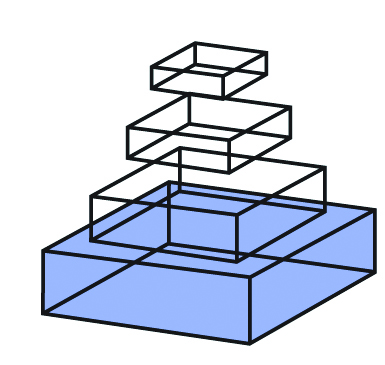
\includegraphics[width=3.5cm]{logo1}% This is a *.jpg file
%\end{center}
% \textbf{\refstepcounter{figure}\label{fig:01} Figure \arabic{figure}.}{ Enter the caption for your figure here.  Repeat as  necessary for each of your figures }
%\end{figure}

%\begin{figure}
%\begin{center}
%
\includegraphics[width=3.5cm]{logo2}% This is an *.eps file
%\end{center}
% \textbf{\refstepcounter{figure}\label{fig:02} Figure \arabic{figure}.}{ Enter the caption for your figure here.  Repeat as  necessary for each of your figures }
%\end{figure}

%\textbf{Figure 1.}{ Enter the caption for your figure here.  Repeat as  necessary for each of your figures.}\label{fig:01}% If you don't add the figures in the LaTeX files, please upload them when submitting the article.

%%% Frontiers will add the figures at the end of the provisional pdf automatically %%%

%%% The use of LaTeX coding to draw Diagrams/Figures/Structures should be avoided. They should be external callouts including graphics.

\end{document}
